\section{Features}

	The current version of \tiger provides the fundamental functaionlities in order to be able to use it as a language workbench. New languages can easily be created and deployed. After a restart they can be used in projects that have the \tiger nature. A \tiger nature can easily be added and removed via a popup menu. The installed DSLs can be configured through the preference pages, as well as the employed transformations. The \tiger editor is an extended version of the Groovy editor and provides keyword coloring for keywords of installed and activated DSLs.
	
	\subsection{Preferences}
	The prefrence pages are an important part of \tiger, since they provide the configuration of registered DSLs. In the main prefrence page (Figure \ref{fig:prefs_main}) the output source folder can be adjusted.
	
	Registered languages can be configured on the languages preference page (Figure \ref{fig:prefs_languages}). DSLs have to be set into activated state in order to use them.	
	The extensions, that indicate which concrete DSL class is responsible for which files of the according extension can be adjusted in the \texttt{Extensions} column. When a DSL is selected its keywords are shown below in the \textit{Declared Keywords of Selected DSL} dialog.
	
	The transformations preference page provides the adjustment of used transformations for the specified resource or DSL (Figure \ref{fig:prefs_transformations}). For each resource and DSL different transformations might be provided. These can be configured using the \texttt{Select Transformations} dialog (Figure \ref{fig:prefs_transformations_selected}). The dialog also shows additional informations about the currently selected transformation in a tray window that can be opened clicking on the additinal information button (Figure \ref{fig:additional_information_button}). The \tiger editor provides keyword coloring for active DSLs. The colors can be configured using the Tigerseye Editor preference page (see Figure \ref{fig:prefs_editor}), where every DSL can be configured seperately and the general keyword coloring can be activated or deactivated.
	
	\begin{figure}
	  \centering
	  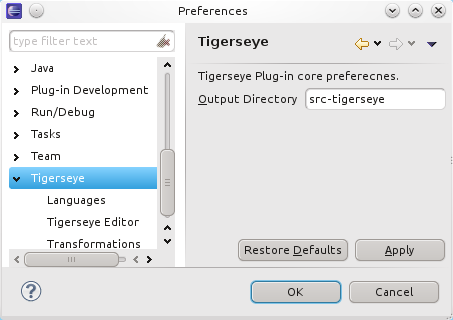
\includegraphics[width=.5\textwidth,keepaspectratio=true]{../pics/preferences_main.png}
	  \caption{Tigerseye Main Preference Page}
	  \label{fig:prefs_main}
	\end{figure}

	\begin{figure}
	  \centering
	  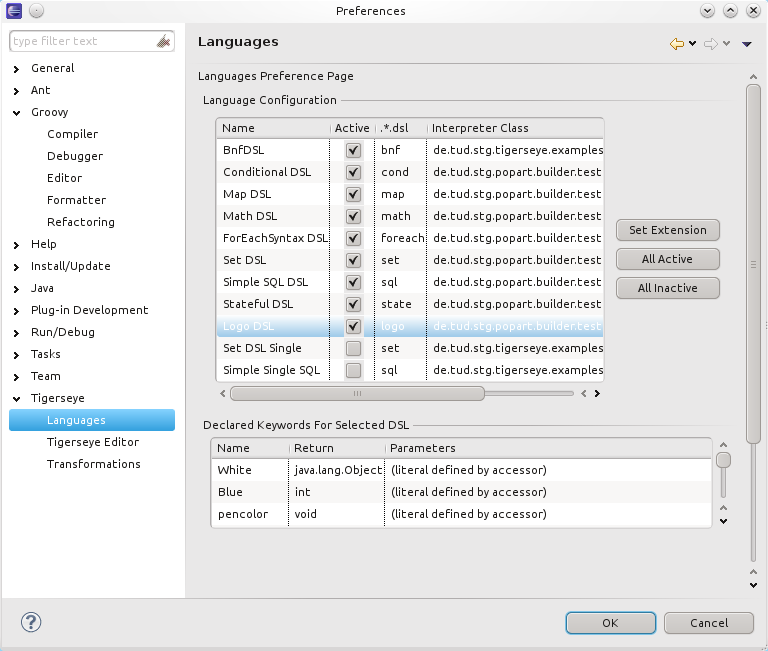
\includegraphics[width=.5\textwidth,keepaspectratio=true]{../pics/preferences_languages.png}
	  \caption{Tigerseye Language Configuration Page}
	  \label{fig:prefs_languages}
	\end{figure}

	\begin{figure}
	  \centering
	  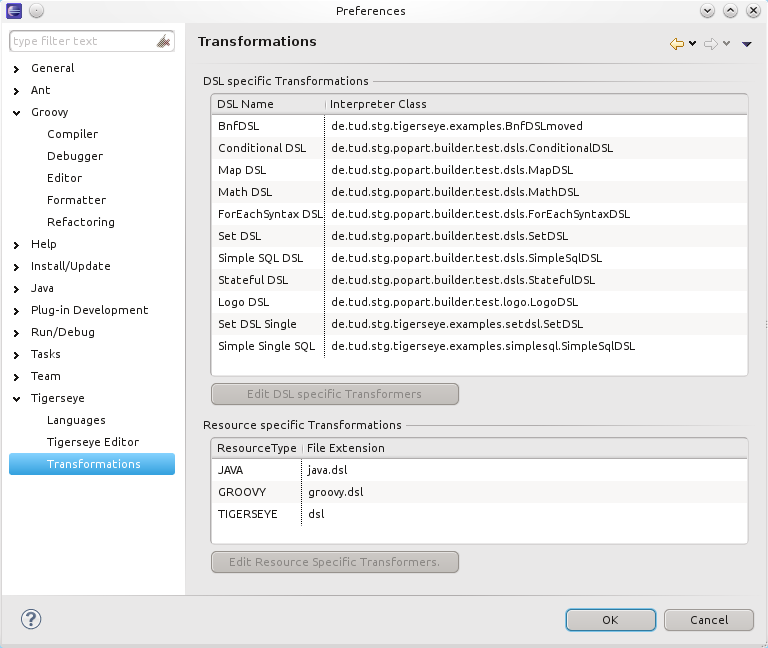
\includegraphics[width=.5\textwidth,keepaspectratio=true]{../pics/preferences_transformations.png}
	  \caption{Tigerseye Transformations Preference Page}
	  \label{fig:prefs_transformations}
	\end{figure}

	\begin{figure}
	  \centering
	  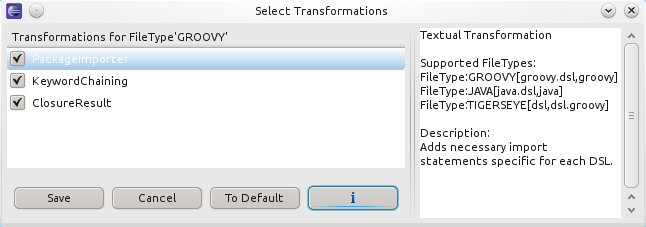
\includegraphics[width=.5\textwidth,keepaspectratio=true]{../pics/preferences_transformations_selected.png}
	  \caption{Tigerseye Transformations Configuration}
	  \label{fig:prefs_transformations_selected}
	\end{figure}

	\begin{figure}
	  \centering
	  
\includegraphics{../pics/additional_information_button.png}
	  \caption{Additional Information Button}
	  \label{fig:additional_information_button}
	\end{figure}

	\begin{figure}
	  \centering
	  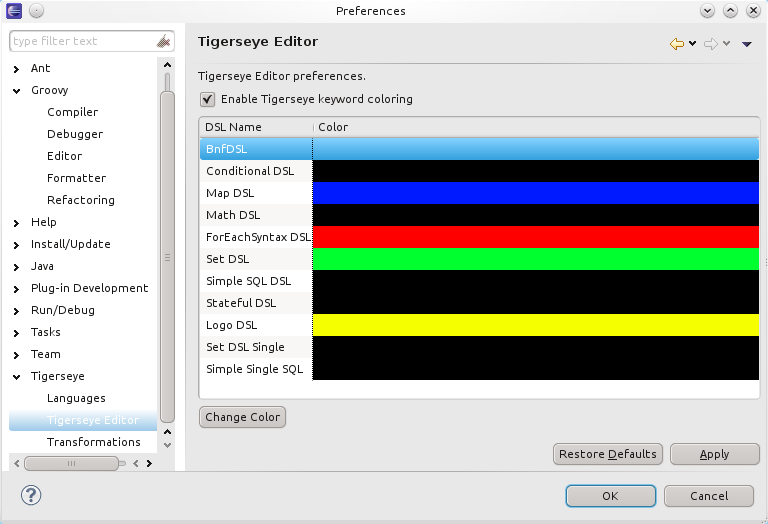
\includegraphics[width=.5\textwidth,keepaspectratio=true]{../pics/preferences_editor.png}
	  \caption{Tigerseye Editor Preference Page}
	  \label{fig:prefs_editor}
	\end{figure}

	\subsection{Add and Remove \tiger Nature}
	  \tiger has additional requirements which will be imported when adding the \tiger nature to a project. The project must have at least the Java nature otherwise the transformation to a \tiger project is not possible. Figure \ref{fig:add_tiger_nature} shows the available popup menu to add the \tiger nature to a project. This will do two things. A seperate source folder will be created into which the translated DSL files will be output (here: \texttt{src-tigerseye}) and a new class path container will be added which contains the runtime libraries (\texttt{popartAnnotations.jar, popart.jar, edslNature.jar}) and the libraries of registered DSLs as well as their dependencies. For example \texttt{de.tud.stg.tigerseye.examples.LogoDSL} and \texttt{de.tud.stg.tigerseye.examples.DSLDefinitions}. Additionally the \texttt{GroovyNature} will be added if not already configured.
	
	\begin{figure}
	  \centering
	  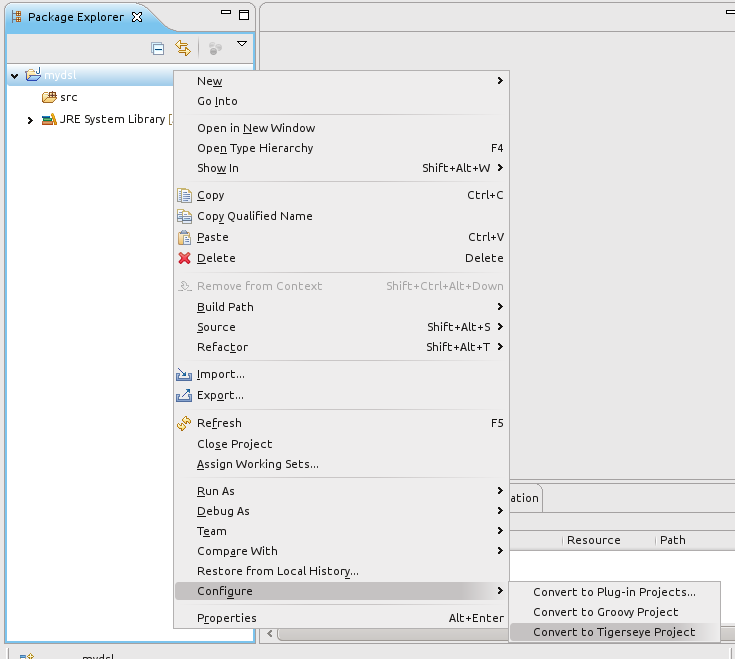
\includegraphics[width=.5\textwidth,keepaspectratio=true]{../pics/convert_to_tigerseye.png}
	  % new_tigesreye_language.png: 525x500 pixel, 93dpi, 14.34x13.66 cm, bb=0 0 406 387
	  \caption{Add the \tiger Nature to a Java Project}
	  \label{fig:add_tiger_nature}
	\end{figure}
	
	\begin{figure}
	  \centering
	  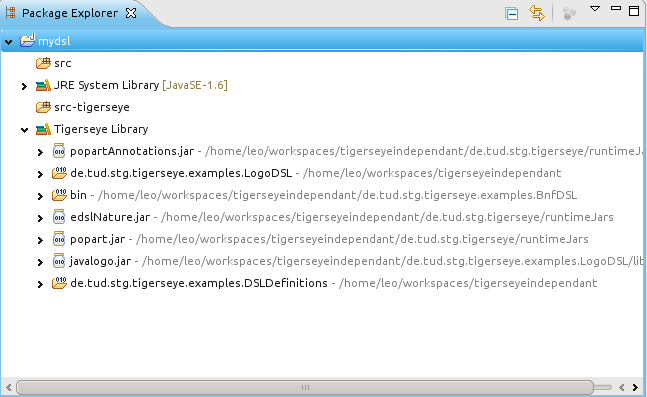
\includegraphics[width=.5\textwidth,keepaspectratio=true]{../pics/tigerseye_dependencies.png}
	  % new_tigesreye_language.png: 525x500 pixel, 93dpi, 14.34x13.66 cm, bb=0 0 406 387
	  \caption{\tiger Dependencies}
	  \label{fig:tiger_added_dependencies}
	\end{figure}
	
	\begin{figure}
	  \centering
	  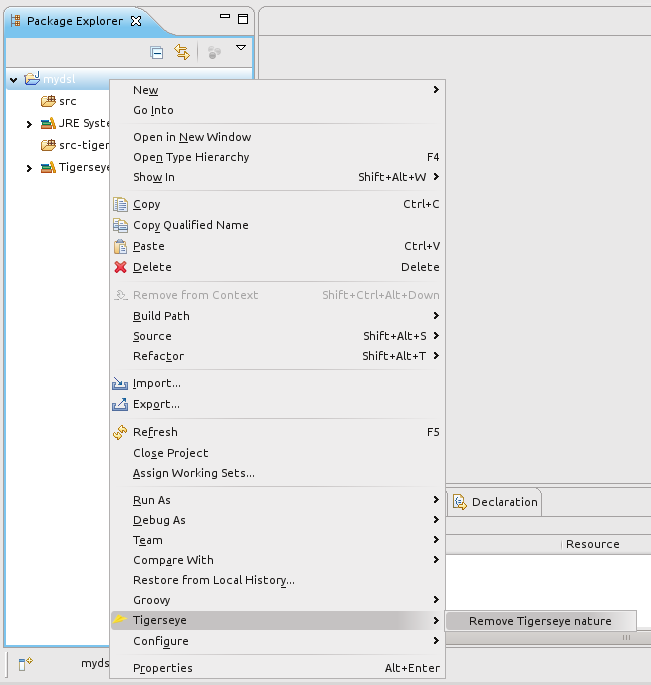
\includegraphics[width=.5\textwidth,keepaspectratio=true]{../pics/remove_tigerseye_nature.png}
	  % new_tigesreye_language.png: 525x500 pixel, 93dpi, 14.34x13.66 cm, bb=0 0 406 387
	  \caption{Remove the \tiger Nature from a Project}
	  \label{fig:remove_tiger_nature}
	\end{figure}
	
	\subsection{\tiger Language Definition Wizard}
	  A new language can be created using the \textit{New Language Wizard}. The Wizard can be accessed via File $->$ New $->$ Other (Figure \ref{fig:new_tiger_lang}). Figure \ref{fig:tiger_lang_definition_page1} shows the first page of the Wizard. There the name of the main language class can be defined. As can be seen in the figure the default package is not a valid package for a language defintion since this will cause problems when trying to use the language within a Java class. Figure \ref{fig:tiger_lang_definition_page2} shows the actual language definition page. There the different literals, operations and structured elements can be added. In Section \ref{sec:examples} the usage of the wizard will be showcased.
	
	\begin{figure}
	  \centering
	  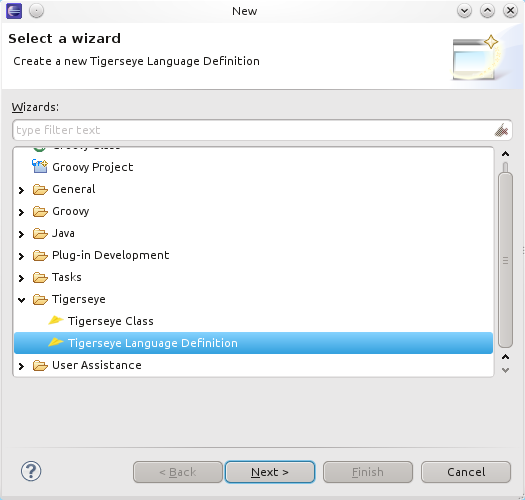
\includegraphics[width=.5\textwidth,keepaspectratio=true]{../pics/new_tigesreye_language.png}
	  \caption{Choosing the New Tigerseye Language Wizard}
	  \label{fig:new_tiger_lang}
	\end{figure}

	\begin{figure}
	  \centering
	  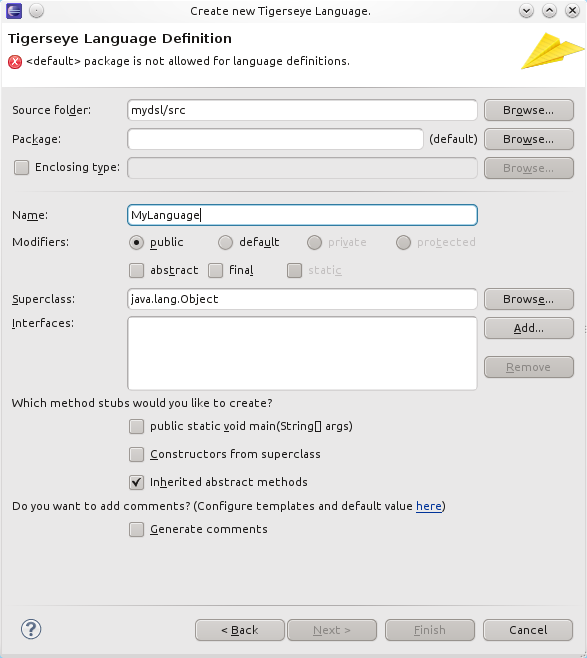
\includegraphics[width=.5\textwidth,keepaspectratio=true]{../pics/tigerseye_language_definition_page1.png}
	  \caption{Tigerseye Language Definition Wizard Page 1}
	  \label{fig:tiger_lang_definition_page1}
	\end{figure}
	
	\begin{figure}
	  \centering
	  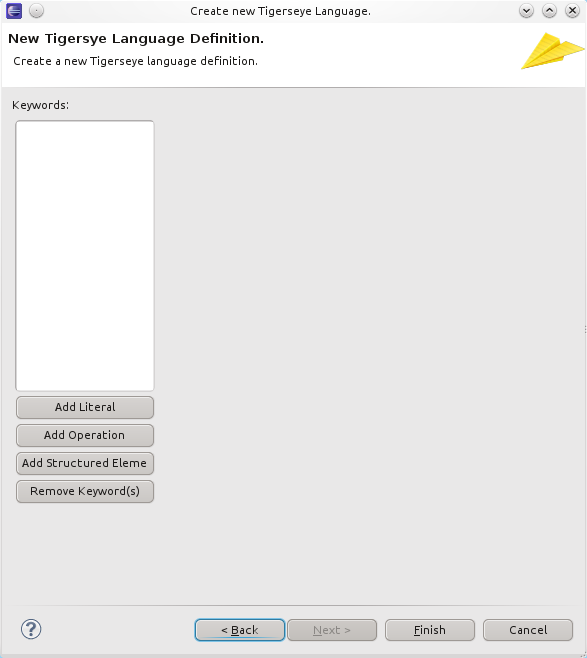
\includegraphics[width=.5\textwidth,keepaspectratio=true]{../pics/tigerseye_language_definition_page2.png}
	  \caption{Tigerseye Language Definition Wizard Page 2}
	  \label{fig:tiger_lang_definition_page2}
	\end{figure}
	
	\subsection{New \tiger Class Wizard}
	  The new \emph{\tiger Class Wizard} enables easy creation of new DSL classes. In Figure \ref{fig:new_tiger_class_page} the Wizard is shown. It is basically an adjusted version of the new Java Class Wizard. Additionally to being able to define the typical class properties a DSL can be chosen which one wishes to use in the class.

	\begin{figure}
	  \centering
	  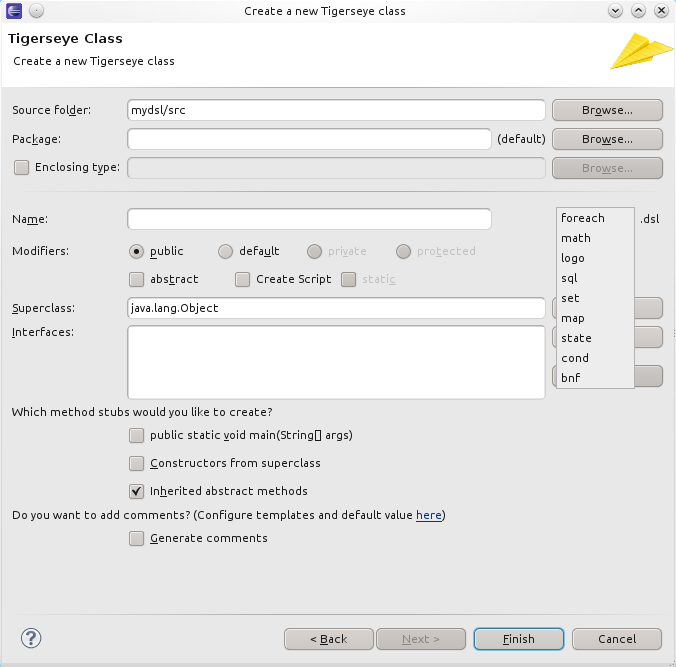
\includegraphics[width=.5\textwidth]{../pics/new_tigerseye_class_wizard.png}
	  \caption{New Tigerseye Class Wizard}
	  \label{fig:new_tiger_class_page}
	\end{figure}	
	
	
	\subsection{Launch Tigerseye DSL}
	  A \tiger1 DSL can be launched using the launch shortcut or via the \textit{Run Configurations} dialog. Figure \ref{fig:launch_shortcut} shows a launch using a launch shortcut. Figure  \ref{fig:launch_run_configurations_dialog} shows the launch via the \emph{Run Configurations Dialog}. There a new launch can be configured or a previous launch adjusted. On the \emph{Tigerseye} tab the project from which a DSL will be launched as well as the dsl file to launch can be chosen. When using the launch shortcut the Groovy default launch configuration is assumed which will set additional classpath properties. Later these can be modified using this dialog.
	
	\begin{figure}
	  \centering
	  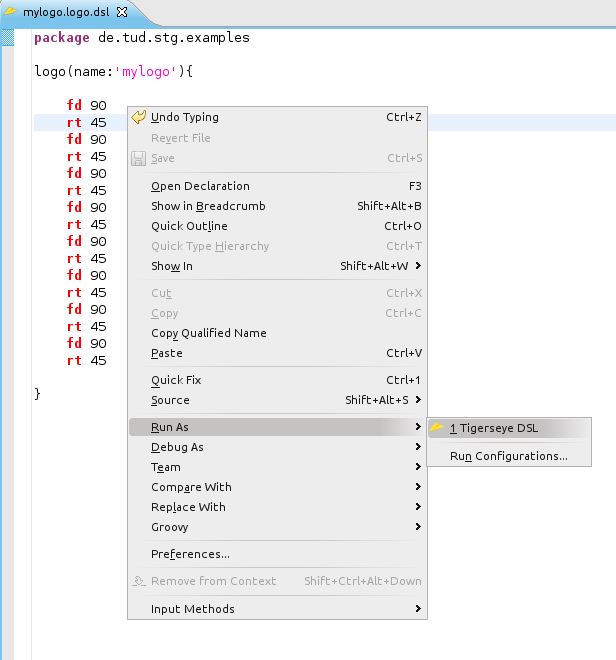
\includegraphics[width=0.5\textwidth]{../pics/launch_shortcut.png}
	  \caption{Launch via Context Menu}
	  \label{fig:launch_shortcut}
	\end{figure}

	\begin{figure}
	  \centering
	  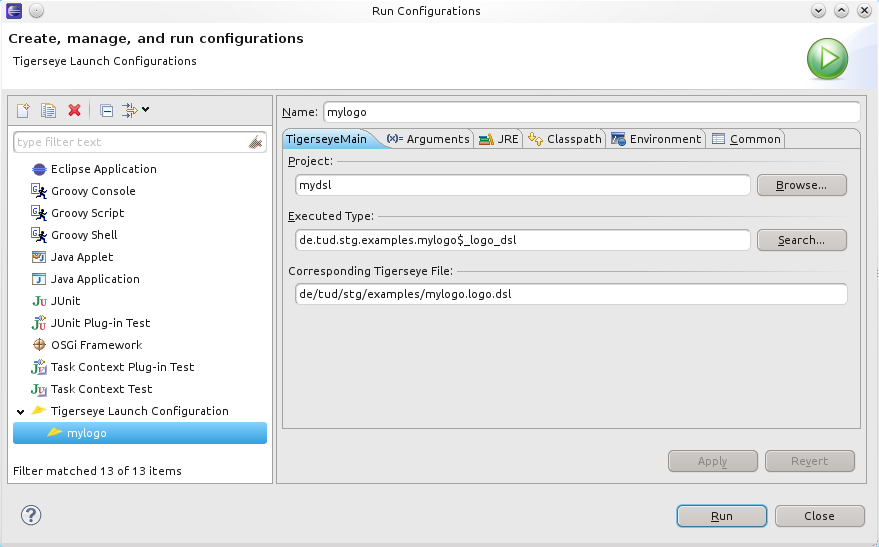
\includegraphics[width=.5\textwidth]{../pics/launch_run_configurations_dialog.png}
	  \caption{Launch via the Run Configurations Dialog}
	  \label{fig:launch_run_configurations_dialog}
	\end{figure}
 
